% !TeX root = Thesis.tex

\chapter{Related~Works}
\label{chap:related_works}

In this chapter, we review prior works on two topics related to our research: \nameref{sec:3d_representations} and \nameref{sec:representation_learning_architectures}.

\section{3D~Representations}
\label{sec:3d_representations}

There are a multitude of methods for digitally representing a 3D volume. Any representation can be used in machine learning, but each has different benefits and challenges. In this section, we discuss the machine learning applications of the five most common 3D representations in the literature.


\subsection{Point~Cloud}
\label{subsec:point_cloud}

\begin{figure}[ht]
	\centering
	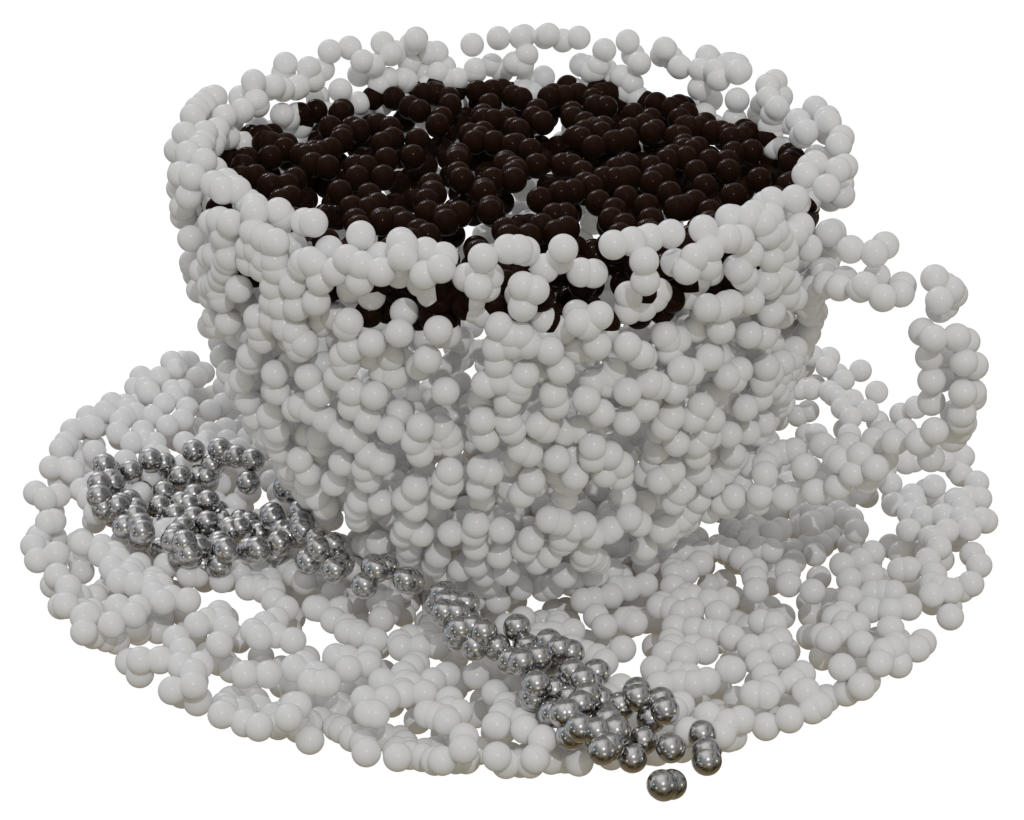
\includegraphics[scale=0.2]{Images/Point Cloud Cup}
	\caption{Point cloud representation of a coffee cup.}
	\label{fig:point_cloud_cup}
\end{figure}

A point cloud is set of unordered 3D coordinates sampled from an object's surface. Point clouds are unstructured and lack topological data~\cite{Xiao2020}. However, this simplicity makes it easy to acquire point clouds using 3D scanning technologies such as lidar and photogrammetry~\cite{Leberl2010}. Photogrammetry is an algorithm that uses multiple photos taken from different angles to triangulate points on a surface. A photogrammetry scan can be performed with even a smartphone, greatly increasing the accessibility of point cloud scans~\cite{Micheletti2015}.

Despite its accessibility, point clouds didn't see use in 3D learning techniques until 2017~\cite{Xiao2020}. Extracting features from point clouds is a challenge since the points are unordered, yet analyzing the proximity between neighboring points is crucial. The points cannot be sorted beforehand because the order would be inconsistent across multiple scans of the same object~\cite{Qi2017}. The 2017 work PointNet~\cite{Qi2017} is first to tackle this challenge. The PointNet architecture directly extracts features from a point cloud using Multi-Level Perceptrons (MLPs) in order to solve the problems of shape classification and part segmentation. The encoder network is composed of two transform layers, two MLP subnetworks, and a max pooling layer. The transform layers align the features to make the model invariant to rigid transformations such as translation, rotation, and scaling. The first MLP network takes an $n$x3 input matrix containing the coordinates of $n$ points. This network analyzes the neighbors of each point and encodes the local structure features into an $n$x64 vector. The local features are then fed through a second MLP network and a max pooling layer to generate a 1x1024 global feature vector. A max pooling layer was chosen because it is a symmetric function that ignores the permutations of the input poitns. The shape classification network analyzes just the global features while the part segmentation network analyzes both the local and global features~\cite{Qi2017}. PointNet is the first work to show that features can be extracted directly from point clouds and laid the foundation for many subsequent works.

The follow up works SpiderCNN~\cite{Xu2018}, PointCNN~\cite{Li2018}, and PointConv~\cite{Wu2019} implement Convolutional Neural Networks (CNNs) instead of MLPs to encode points. While the PointNet architecture has one local feature layer and one global feature layer, CNNs specialize in extracting many features layers of varying resolution. The increased number of feature layers enables CNN based models to better analyze hierarchical data than MLP based models. As a result, SpiderCNN, PointCNN, and PointConv have all surpassed PointNet in both shape classification and part segmentation accuracy~\cite{Wu2019}.

Further works~\cite{Fan2017, Achlioptas2018} have demonstrated that deep learning models can be trained to reconstruct an input as a point cloud. The model presented in~\cite{Fan2017} takes a 2D image of an object as input and generates a cloud of 1024 points to represent its surface. CNN networks are used for both the image encoder and point cloud decoder. Not only can the model reconstruct 3D shapes from images, but it can also infer the missing parts of an input. \cite{Achlioptas2018} uses the PointNet encoder as a base and adds a fully connected MLP decoder network to generate point clouds. The work experiments with two training strategies. The first architecture is an autoencoder network trained using a loss function. The second architecture keeps the same generative network and introduces a discriminator network to form a Generative Adversarial Network (GAN). Both architectures demonstrate strong results but the autoencoder performes slightly better than the GAN.

Although point clouds only offer a sparse approximation of a surface, their low-dimensionality proves useful in efficiently learning 3D features.


\subsection{Polygon~Mesh}
\label{subsec:polygon_mesh}

\begin{figure}[ht]
	\centering
	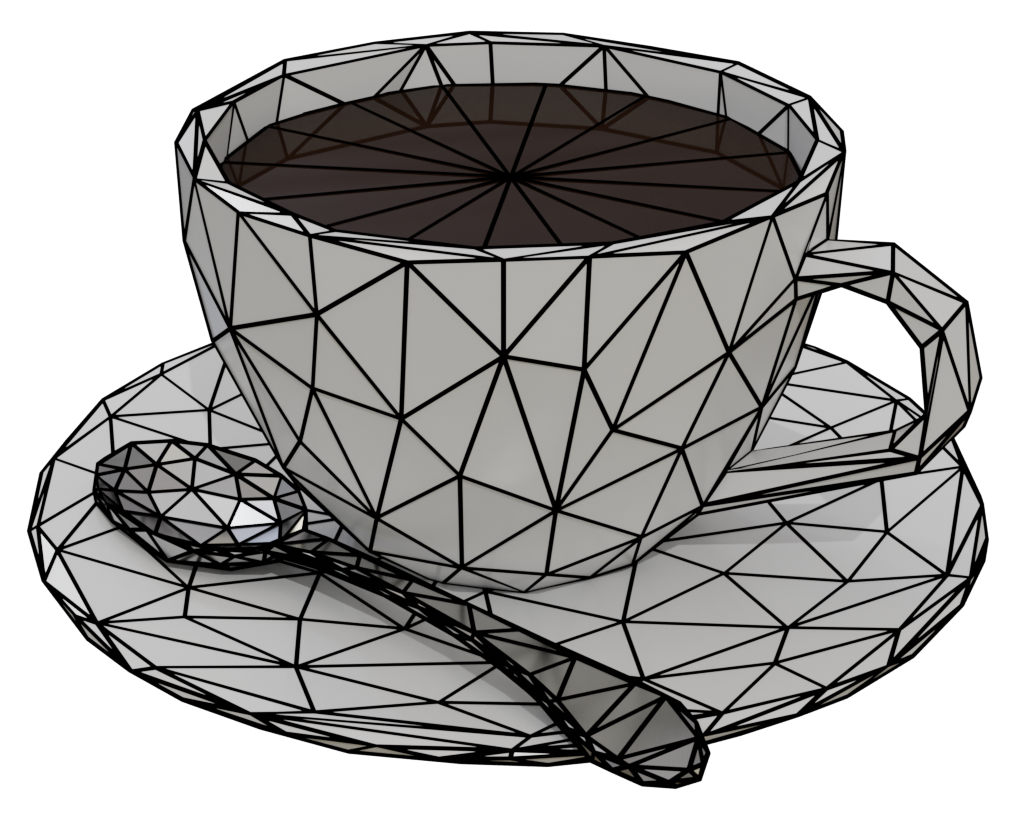
\includegraphics[scale=0.2]{Images/Mesh Cup}
	\caption{Triangle mesh representation of a coffee cup. The black lines depict the connecting edges between vertices.}
	\label{fig:mesh_cup}
\end{figure}

Mesh-based models consist of vertices connected by flat polygonal faces. Unlike point clouds, meshes can represent topology and surface details~\cite{Xiao2020}. Polygon meshes are the most popular 3D representation for use in computer graphics because they can be quickly rendered into images~\cite{Watt1996}. Another unique benefit is that meshes are easy to deform and animate~\cite{Wang2018}. These qualities make mesh-based models ideal for use in video games, virtual reality, and film~\cite{Nash2020}. One issue is that meshes cannot be directly acquired using 3D scanners. This is easily circumvented by using surface reconstruction techniques to generate meshes from point cloud scans~\cite{Yuan2022}.

The prevalence of polygon meshes has motivated many mesh-based deep learning models. Since the structure of a polygon mesh is complex, these models adopt unique architectures to simplify the problem. To directly process polygon meshes, models such as FeaStNet~\cite{Verma2018} and MeshCNN~\cite{Hanocka2019} employ Graph Convolutional Networks (GCN). A mesh can be seen as a directed graph of interconnected nodes. This enables graph-based methods such as GCN to directly consume meshes as input. While a traditional CNN applies filters to a group of pixels in an image, a GCN applies filters to a group of nodes or edges in a graph. Like CNNs, GCNs support pooling operations to extract features from a mesh~\cite{Verma2018}. In addition to pooling operations, MeshCNN introduces graph-based unpooling operations to increase the resolution of a mesh.

Techniques to generate meshes are more varied. AtlasNet~\cite{Groueix2018} uses MLPs to reconstruct a point cloud out of 2D meshes. The model starts with flat planes  as a template. The planes are then deformed to represent the surface of the point cloud. At the end, all the planes are stitched together. This papier-m\^{a}ch\'{e} approach is efficient but does not produce a continuous surface~\cite{Groueix2018}. Pixel2Mesh~\cite{Wang2018} and Point2Mesh~\cite{Hanocka2020} both deform a 3D template mesh through cascaded refinement to represent the input. Instead of a flat plane, Pixel2Mesh and Point2Mesh start with a sphere encompassing a point cloud. The template is then deformed in a coarse-to-fine manner with the resolution of the template mesh increasing each iteration. Starting with a lower resolution allows the model to quickly build a rough approximation of the shape. Then the resolution is gradually increased to allow for more fine adjustments. Working with the minimum required resolution for any given iteration greatly improves the efficiency of these models. Unlike AtlasNet, Pixel2Mesh and Point2Mesh are guaranteed to generate manifold surfaces since the initial template shape is manifold. A limitation of current deformation based works is that the output is always a genus 0 shape. The models have no means to merge or remove geometry to represent holes~\cite{Wang2018, Hanocka2020}.

PolyGen~\cite{Nash2020} takes the most direct approach in generating 3D meshs. A vertex generation network predicts a variable number of vertices to represent the input. The vertices are then fed to a face generation network that best connects the vertices with edges and faces. Both networks are implemented as transformers~\cite{Nash2020}. Similar to a Long short-term memory (LSTM) network or a Recurrent Neural Network (RNN), a transformer consumes and produces sequential data. However unlike  an RNN or LSTM, the innovative architecture of a transformer network allows the outputs to be computed parallel. This not only makes training and using the network faster, but also enables longer input and output sequences~\cite{Vaswani2017}. Transformers have a fixed output size, so the authors include a stopping token to the output parameters of the vertex network to allow for variable size meshes. The maximum resolution of the output mesh is 1200 vertices and 800 faces. Because Polygen directly generates meshes, it can represent geometric shapes with far fewer polygons than similar works. The biggest limitation of PolyGen is its small output resolution. The computational cost of a transformer network increases quadratically with the size of the network. Despite some optimizations, the transformer networks are too inefficient at scale to generate more detailed meshes. Due to this limitation, PolyGen is focused on representing simple geometric shapes with the minimum number of polygons~\cite{Nash2020}.

The polygon mesh is one of the most convenient formats. However, deep learning models struggle to generate meshes due to their non-Euclidean nature. Existing works are either limited in the type geometry they can generate or suffer from a small output resolution.

\newpage


\subsection{Occupancy~Grid}
\label{subsec:occupancy_grid}

\begin{figure}[ht]
	\centering
	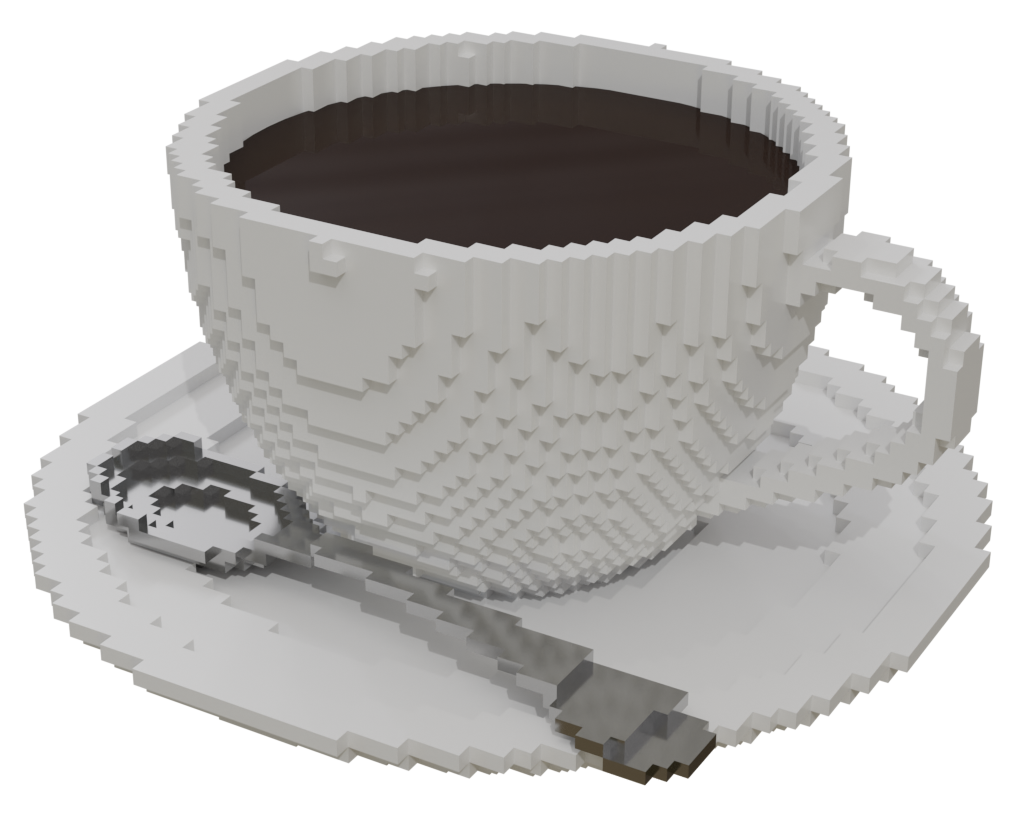
\includegraphics[scale=0.2]{Images/Voxel Cup}
	\caption{Voxel grid representation of a coffee cup.}
	\label{fig:voxel_cup}
\end{figure}

An occupancy grid, also known as a voxel grid, discretizes 3D space into a regular grid of voxels. Each voxel stores a probability that it is occupied or vacant. A volume can be represented as the set of all cells it occupies. There are several variations of occupancy grids that store different values in the voxels. A binary occupancy grid stores occupancy information as a binary value instead of a probability~\cite{Konolige1997}. Some variations also add a parameter for voxels with an unknown state~\cite{Ahmed2018}.

The first work to apply occupancy grids as a 3D representation in the context of deep learning was 3D ShapeNets~\cite{Wu2015}. The ShapeNets model takes a four-channel RGB-D depth image as input. In addition to red, greed, and blue color values, RGB-D images store the distance from the camera to the scene in each pixel. The RGB-D images are converted to an occupancy grid as a pre-processing step. The input occupancy grid dimensions are $30^3$ voxels with 3 voxels of padding on all sides of the object. In a single-view RGB-D image, parts of the scene will be occluded. To accommodate for this, the authors add a third ``occluded'' state to each voxel in addition to the ``vacant'' and ``occupied'' states~\cite{Wu2015}.

The voxel representation is then fed into a modified Deep Belief Network (DBN) that the authors call a Convolutional Deep Belief Network (CDBN)~\cite{Wu2015}. DBNs offer several advantages over traditional neural networks, including more efficient learning and the ability to pre-train on unlabeled datasets. A DBN is composed of multiple Restricted Boltzmann Machines (RBMs) that are stacked such that the hidden layer of one RBM becomes the visible layer of the next~\cite{Aljabery2020}. Each RBM layer is trained to represent the data in the previous layer. Earlier RMBs learn low level features while later RBMs learn high level features. The features encoded in the last layer of the DBN can then be decoded using other machine learning techniques~\cite{McAfee2008}. The ShapeNets CDBN architecture (Convolutional Deep Belief Network) adds convolution operations to a standard DBN to make it compatible with 3D inputs. The ShapeNets model was trained using contrastive divergence for unsupervised pre-training and a method similar to the wake-sleep algorithm for supervised fine-tuning. The resulting feature vector is then fed to a Support Vector Machine (SVM) to perform shape classification~\cite{Wu2015}.

VoxNet~\cite{Maturana2015} improves upon ShapeNet with a 3D CNN architecture. It simple in theory to extend a 2D image processing CNN to handle 3D occupancy grids. In practice, however, the increased memory and computational requirements added by the extra spacial dimension pose a challenge. Due to these restrictions, the VoxNet architecture limits the input size to a grid of 32x32x32 voxels. The voxel input is fed through a network consisting of two convolution layers, one pooling layer, and two fully-connected layers to produce class label predictions. To better capture fine details, VoxNet implements a multiresolution architecture by combining two of these convolutional networks. Both networks are identical but are fed different inputs. The voxels in the coarse input represent a volume of $0.2m^3$ while the voxels of the fine input represent $0.1m^3$. The outputs of both networks are then combined to produce a final class prediction. The VoxNet architecture is easier to train than ShapeNet since it has ten times fewer parameters. And VoxNet also outperforms ShapeNet in classification accuracy~\cite{Maturana2015}.

Seeing as the main drawback to occupancy grids is the inefficiency, several works have focused on optimization. The authors of LightNet~\cite{Ye2016} optimize using a multi-task learning approach. This is a technique where a single model is trained to solve multiple tasks at once. In doing so, the model avoids overfitting and learns to extract general features. In the case of LightNet, the model is trained to predict the class and orientation of an input volume. LightNet enjoys performance improvements over VoxNet but is still contained to an input resolution of $32^3$ voxels~\cite{Ye2016}. 

Instead of optimizing the model directly, Octree Generating Networks (OGN)~\cite{Tatarchenko2017} optimize the data format. The works we've discussed thus far store each voxel of the occupancy grid in a dense array. Continuous arrays are simple to work with but have increased dimensionality due to redundant data. OGN compresses the occupancy grid data using an octree data structure. The root node contains 8 octants encompassing the entire volume. Each of the 8 octants is a child node that either subdivides the volume further or terminates in a leaf node. This spacial partitioning scheme efficiently summarizes groups of similar voxels and reduces the format size. The octree format is used for both the input and output of the OGN architecture. OGN is a self-supervised convolutional autoencoder network trained to reconstruct the input occupancy grid. The data compression enables a massive jump to a resolution of $512^3$ voxels on consumer hardware. A downside to this approach is the complexity needed to support octrees. The octree structure is stored in a hash table for quick lookup. If this hash table is not available during runtime, the performance of the model significantly decreases. And despite the large optimization, OGN can take over a week to train at higher resolutions~\cite{Tatarchenko2017}.

Occupancy grids provide rich volumetric data for object classificaiton and reconstruciton tasks. While prior works have used occupnacy grid representations with great success, the computational cost limits their applications.

\newpage


\subsection{Images}

\begin{figure}[ht]
	\centering
	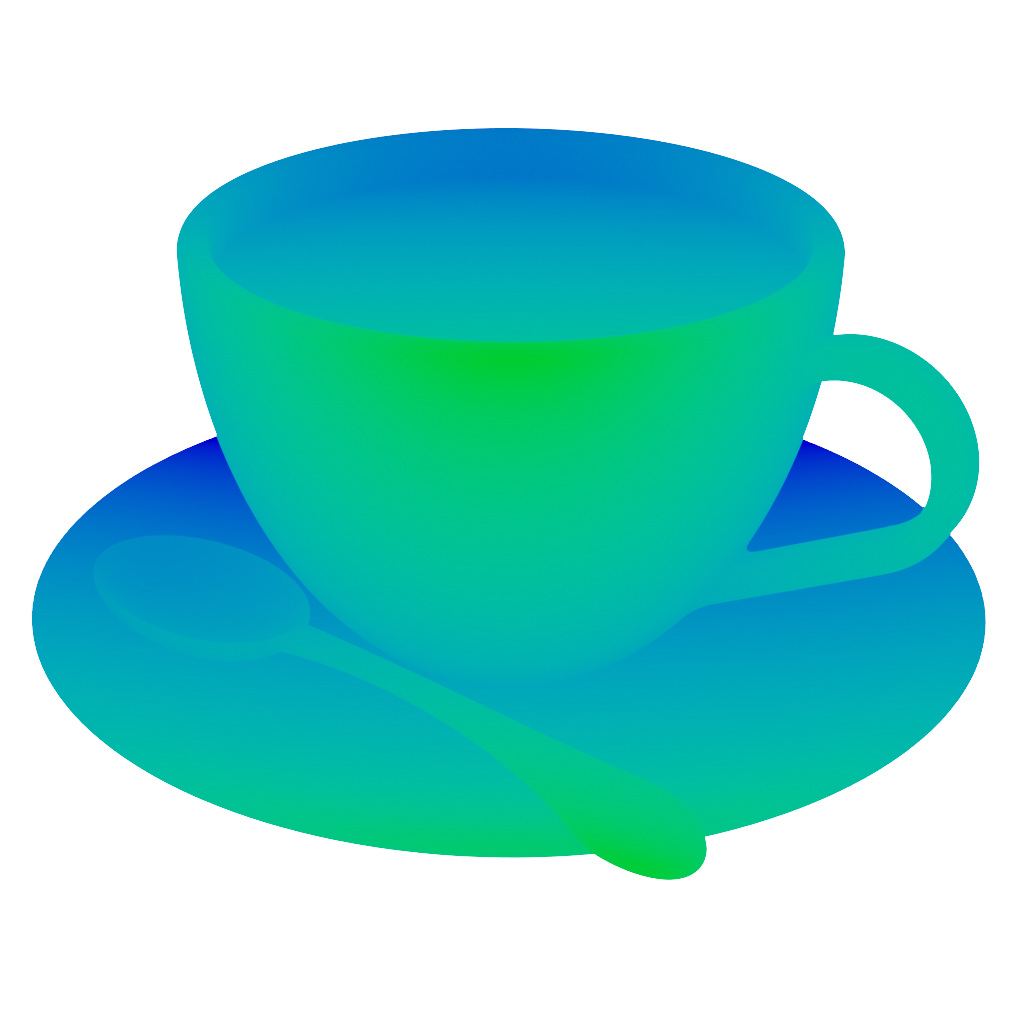
\includegraphics[scale=0.2]{Images/Depth Map Cup}
	\caption{Depth map representation of a coffee cup. Points closer to the camera are colored green and points further from the camera are colored blue.}
	\label{fig:depth_map_cup}
\end{figure}




\subsection{Implicit~Surface}
\label{subsec:implicit_surface}

\begin{figure}[ht]
	\centering
	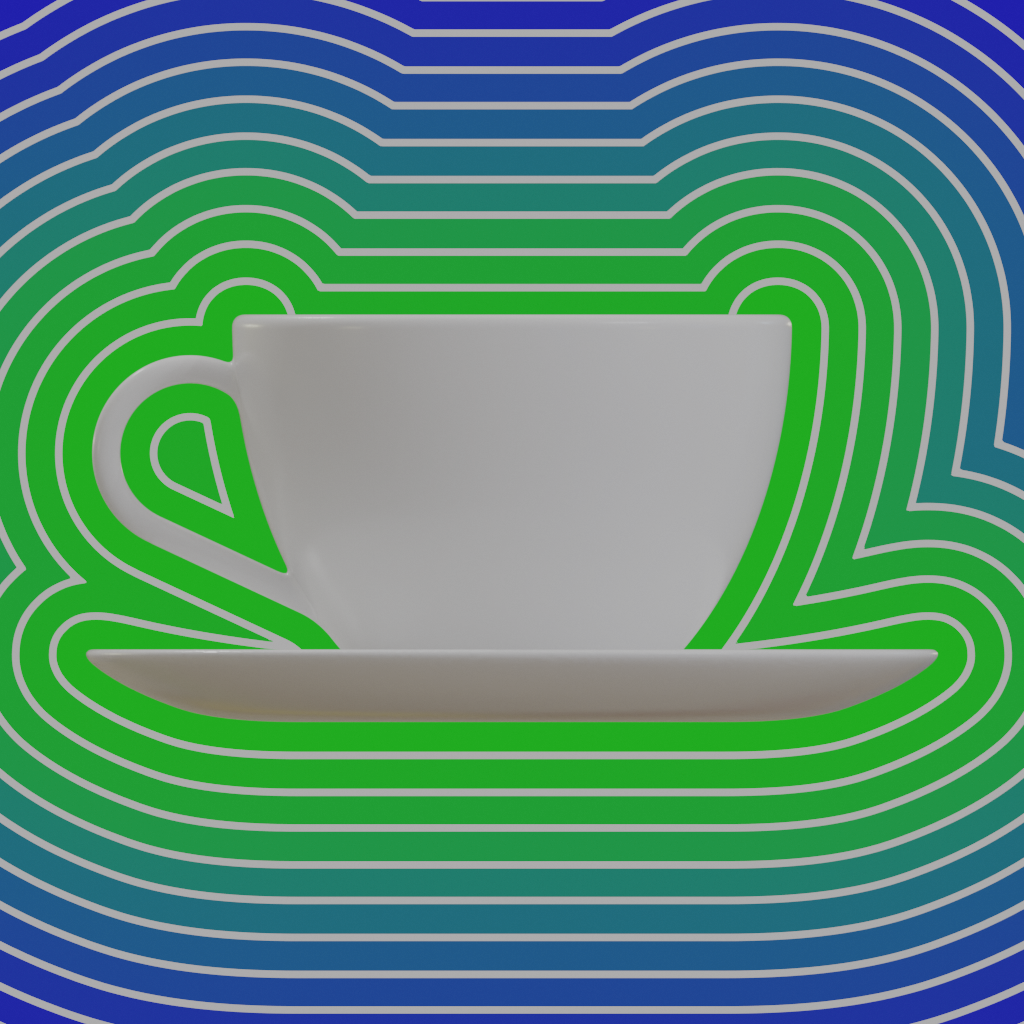
\includegraphics[scale=0.2]{Images/SDF Cup}
	\caption{Visualization of an SDF representing a coffee cup. Points close to the surface are drawn green and points far from the surface are drawn blue. Each white contour line consists of points that are equidistant from the surface.}
	\label{fig:sdf_cup}
\end{figure}

\subsection{Structured~Representation}
\label{subsec:structured_representation}

\begin{figure}[ht]
	\centering
	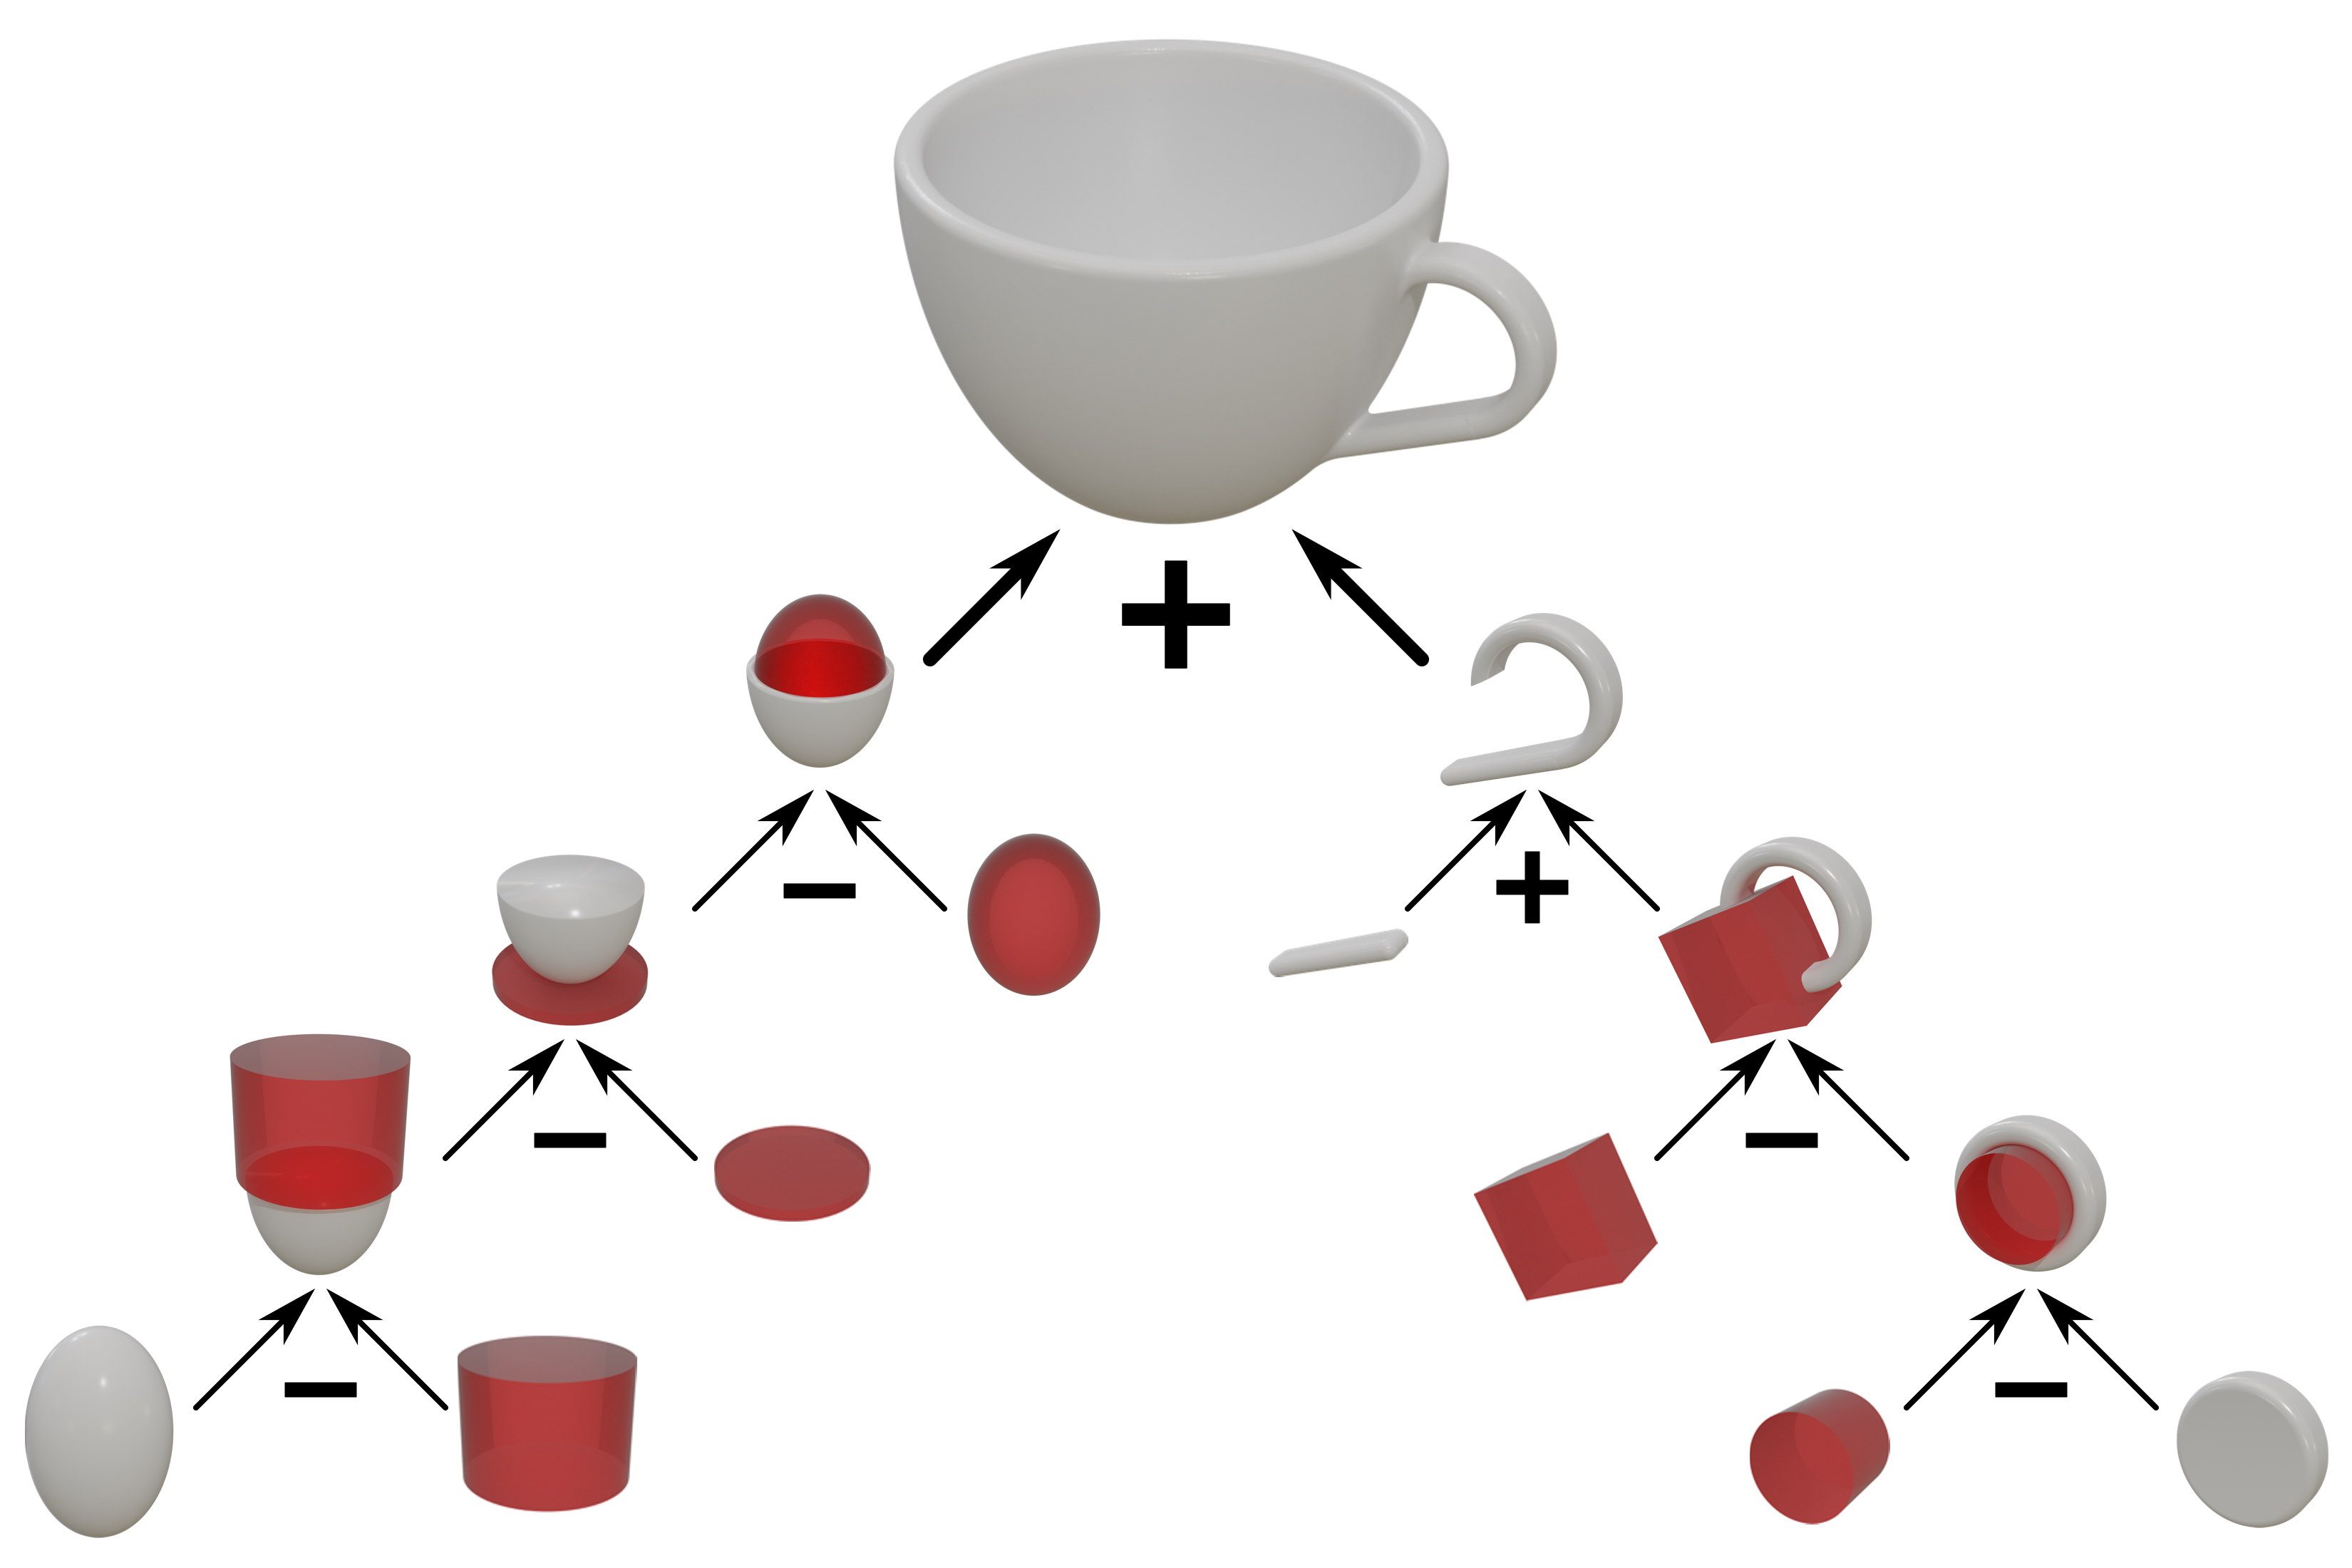
\includegraphics[scale=0.5]{Images/CSG Cup}
	\caption{The CSG tree of a coffee cup. The leaves of the tree are SDF primitives which are combined through union (+) and difference (-) operations. The primitives being subtracted are colored red.}
	\label{fig:csg_cup}
\end{figure}


\section{Representation~Learning~Architectures}
\label{sec:representation_learning_architectures}

Test

\subsection{Generative~Adversarial~Network}
\label{subsec:generative_adversarial_networks}

Test

\subsection{Autoencoder}
\label{subsec:autoencoders}

Test

\subsection{Cascaded~Refinement}
\label{subsec:cascaded_refinement}

Test